\documentclass[bibliography=totocnumbered]{scrartcl}
\usepackage{imakeidx}
\usepackage{ragged2e}
\usepackage{setspace} % Um den Zeilenabstand zu ändern.
\usepackage{gensymb}
%\usepackage{authblk}
% \usepackage{minitoc} % for the chpaters
\usepackage{wasysym}
%\usepackage{SI}
\usepackage{array} % Verwendung von Matrizen
\usepackage{booktabs} % Schöne Tabellen beziehungsweise sie sehen damit professioneller aus.
\usepackage{tabulary} % Ähnlich wie tabularx, ermöglicht aber das ändern der Ausrichtung der Spalten.
\usepackage{tabularx} % Tabellen mit automatischen Zeilenumbruch.
\usepackage{enumitem}
\usepackage{physics}
\usepackage[T1]{fontenc}% fontec und inputenc ermöglichen
\usepackage{graphicx}%Für Grafiken
\usepackage{rotating} % lässt Grafiken rotieren
\usepackage{mathtools}% mathematische Werkzeuge
\usepackage{amsmath}% Mathetools
\usepackage{amsfonts}% Mathetools
\usepackage{amssymb}% Symbole wie Natürliche Zahlen
\usepackage{geometry}
%\usepackage{bibtex} 
\usepackage{tablefootnote}% Fußnoten in Tabellen
\usepackage{float}% für eingebundene Bilder
\usepackage{fancyhdr} % Seiten schöner gestalten, insbesondere Kopf- und Fußzeile
\usepackage{ulem} 
\usepackage{dcolumn}% Align table columns on decimal point
\usepackage{bm}% bold math
\usepackage[ngerman]{babel} % Worttrennung nach der neuen Rechtschreibung und deutsche Bezeichnungen. babelfunktion wird wegen Literatur gebraucht.
\usepackage{subfloat} % Was macht diese Packet?
\usepackage{caption} % Unter-/Überschriften für Bilder, Grafiken und Tabellen
\usepackage{subcaption}
\usepackage{txfonts}
\usepackage{titling}% Titel
\usepackage[style=alphabetic]{biblatex} %biblatex mit alphabetic laden. alphbetic=Zitationsstil
\usepackage{bookmark}
\usepackage[printonlyused]{acronym}
\usepackage{amsthm}
\usepackage{pdfpages}
\usepackage{tikz}
\usepackage[siunitx,americanvoltages, europeanresistors,americancurrents]{circuitikz}
\usepackage{listings}
\usepackage{abstract}
\usepackage[per-mode = fraction]{siunitx}
\usepackage{hyperref}
\newcommand{\R}{\mathbb{R}} % reelle Zahlen
\newcommand{\N}{\mathbb{N}} % natürliche Zahlen
\newcommand{\C}{\mathbb{C}} % komplexe Zahlen
\newcommand{\Q}{\mathbb{Q}} % rationale Zahlen
\newcommand{\Z}{\mathbb{Z}} % ganze Zahlen
\newcommand{\F}{\mathbf{F}} % Kraft
\newcommand{\E}{\mathbf{E}} % Energie
\newcommand{\V}{\mathbf{v}} % Geschwindigkeit
\newcommand{\B}{\mathbf{B}} % magnetischer Fluss
\newcommand{\J}{\mathbf{j}} % Stromdichte ?
\newcommand{\D}{\mathbf{D}} % elektrische Induktion
\newcommand{\HH}{\mathbf{H}} % magnetische Feldstärke
\newcommand{\M}{\mathbf{M}} % Magnetisierung
\newcommand{\p}{\mathbf{P}}
\newcommand{\rr}{\mathbf{r}}
\newcommand{\vp}{\varphi}
\newcommand{\ve}{\varepsilon}
\newcommand{\vcc}[1]{\left(\begin{matrix}#1\end{matrix}  \right)}
\newcommand{\m}[1]{\left\lbrace #1\right\rbrace}
\newcommand{\los}{\noindent\textbf{Lösung}:}
\newcommand{\rang}[2]{\text{Rang}(#1)=#2}
\newcommand{\vpe}{\frac{1}{4\pi\ve_0}}
\newcommand{\qvpe}{\frac{q}{4\pi\ve_0}}
\newcommand{\geg}{\ac{geg.}}
\newcommand{\ges}{\ac{ges.}}

\newcommand{\kommando}[1]{$\backslash$\textit{#1}}
\newcommand{\com}[1]{$\backslash$\textit{#1}$\left\lbrace\ldots\right\rbrace$}
\newcommand{\Com}[2]{$\backslash$\textit{#1}$\left\lbrace #2\right\rbrace$}
\newcommand{\NeuKommando}[2]{$\backslash \textit{#1} \left\lbrace \backslash \textit{#2}\right\rbrace$}
\newcommand{\latex}{\LaTeX $\;$}


% si unitx
\DeclareSIUnit\litre{l}

\hypersetup{
	colorlinks=true,
	linkcolor=blue,
	filecolor=magenta,      
	urlcolor=cyan,
	citecolor=lime!50!black,
	filecolor=red
}
%\addbibresource{} %Bibliographiedateien laden
\addbibresource{bib.bib}

\geometry{a4paper, left=25mm, right=25mm, top=30mm, bottom=30mm}
\lhead{\thedate}
\rhead{GPR}
\lhead{\thetitle}
\pagestyle{fancy}

\usetikzlibrary{patterns}
\usetikzlibrary{3d}
\makeindex[title=Stichwortverzeichnis,intoc
,options= -s Index-Formatierung.ist
]
\author{Ben J. F.}
\allowdisplaybreaks

\lstset
{ %Formatting for code in appendix
    basicstyle=\footnotesize,
    numbers=left,
    stepnumber=1,
    showstringspaces=false,
    tabsize=2,
    breaklines=true,
    breakatwhitespace=false,
}




\title{M2 - Trägheitsmoment}
\date{04.05.2021}
\rfoot{M2}

\begin{document}
	\newgeometry{left=14mm, right=13.5mm, top=60mm, bottom=30mm}
	\begin{titlepage}
		\begin{center}
			{\huge{P6.1 Grundpraktikum I}}\\\vspace*{15mm}
			{\huge{\textbf{\thetitle}}}\\\vspace*{20mm}
			{\theauthor}\\\vspace*{10mm}
			{\thedate}\\\vspace*{20mm}
			
			\vspace{1.5cm}
			\begin{abstract}
				Wir wollen experimentel das Trägheitsmoment eines Drehtisches und die Trägheitsmomente zweier Hauptträgheitsachsen eines verstellbaren Zylinders ermitteln. Für das Trägheitsmoment des Tisches haben wir folgendes Ergebnis: $ J_{Tisch} =(5.8\pm 0.2)10^{-4} \textit{ mkg}^{2}$. Die Ergebnisse für die beiden Haupträgheitsmomente des Zylinders sind nicht vertrauenswürdig.
			\end{abstract}
			
			
		\end{center}
	\end{titlepage}
	\makeatother
	\restoregeometry
	\newpage
	
	\tableofcontents
	\listoffigures 
	\listoftables
	\newpage

	
	
	\section{Versuchsbeschreibung}
	% Versuchziel: Was will ich mit dem Versuch erreichen?
	% Aufgabenstellung
	% theoretische Einführung: Wie sieht die Physik dahinter aus (Knapp fassen)? Welche Formeln verwende ich? Wie ist der Versuch aufgebaut (Skizze, Abbildungen etc)? Welche Einheiten kommen vor?
	\subsection{Bestimmung des Trägheitsmoments von einem Drehtisch}
	\begin{figure}[!ht]
		\centering									% Bild Zentrierung
		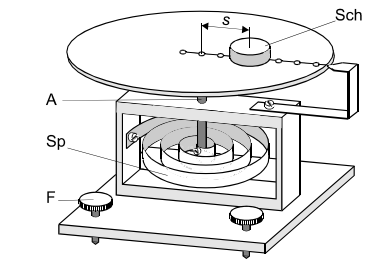
\includegraphics[width=200pt]{fotos/gpr1/Drehtisch.png}			% einfügen des Bildes/ mit width Bildbreite einstellen
		\caption{Drehtisch: F= verstellbare Schraube, A=Drehachse, s=Symmetrieachse, Sp=Schneckenfeder, Sch=Scheibe }							% Bildunterschrift
		\label{Abb.: Drehtisch}							% für Textverweise
	\end{figure}
\begin{equation}\label{eq: T_sq=f(J_z)}
	T^{2}=\dfrac{4\pi^{2}}{D}\left(J_{Z}+J_{T}\right)
\end{equation}
	In diesem Teilversuch ist es das Ziel, das Trägheitsmoment des Drehtisches\footnote{Abb. 1 \ref{Abb.: Drehtisch}} ($ J_{T} $) über eine lineare Regression zwischen der quadrieten Periodendauer $ T^{2} $ und dem zusätzlichen Trägheitsmoment $ J_{Z} $ zu bestimmen.$ ^{\ref{eq: T_sq=f(J_z)}} $ Dabei werden die beiden Regessionsparameter das Richtmoment der Feder $ D $ und $ J_{Tisch} $ sein. Dazu lenken wir den Tisch mehrmals aus. Dabei ist der Tisch in der ersten Messreihe leer. Danach setzen wir eine Scheibe\footnote{Radius: $ (2405\pm2.5)\cdot 10^{-5} $ m, Masse: $ (2453\pm1)\cdot 10^{-4} $ kg} auf den Teller und setzen diese vom Zentrum des Tellers in 6 Schritten an den Rand des Tellers. Bei jedem der 7 eben benannten Schritten messen wir jeweils zweimal die Periodendauer $ T $ über 10 Schwingungen mit einer Stoppuhr. \\
	Das zusätzliche Trägheitmoment $ J_{Z} $ ist über den Steinerschen Satz wie folgt definiert:
	\begin{equation}\label{eq: J_Z1}
		J_{Z}=\dfrac{1}{2}mR^{2}+ms^{2}
	\end{equation}
In $ J_{Z} $ ist auch das Trägheitsmoment der Scheibe enthalten:
\begin{equation}\label{eq: J_sch}
	J_{Sch}=\dfrac{1}{2}mR^{2}
\end{equation}
	Für die Unsicherheiten von $ T^{2} $, $ J_{Z} $ und  $ J_{Tisch} $ verwenden wir die Fehlerfortpflanzung\footcite[vgl][8]{Eichler.2016}, die allgmein definiert als:
	\begin{equation}\label{eq: Fehlerfortpflanzung}
		u_{z}=\sqrt{\left(\dfrac{\partial z}{\partial a}\right)^{2}u_{a}^{2}+\left(\dfrac{\partial z}{\partial b}\right)^{2}u_{b}^{2}+\left(\dfrac{\partial z}{\partial c}\right)^{2}u_{c}^{2}+...}
	\end{equation}
	Für $ T^{2} $ sieht die Fehlerfortpflanzung folgendermaßen aus:
	\begin{equation}\label{eq: u_T_sq}
		u_{T^{2}}=2\dfrac{T}{100}u_{\text{Fehler der Stoppuhr}}
	\end{equation}
	Wir teilen $ T $ durch 100, weil wir über 10 Schwingungen gemessen haben und diese in der Fehlerfortpflanzung quadriert wird.Den Fehler der Stoppuhr, welche in der Glg. (\ref{eq: u_T_sq}) steht ist wie folgt definiert\footnote{Wir verwenden hier den Eichfehler einer Digital-Stoppuhr aus \smartcite[vgl][18]{MullerPG.2007b}}:
	\begin{equation}\label{eq: Fehler Stoppuhr}
		u_{\text{Fehler der Stoppuhr}}=0.01+5\cdot 10^{-4}\cdot T
	\end{equation}
	Fehlerfortpflanzung für $ J_{Z} $:
	\begin{equation}\label{eq: u_J_Z}
		u_{J_{Z}}=\sqrt{\frac{r^{2}}{4}(u_{m}^{2} r^{2}+(2 m   u_{r})^{2})+u_{m}^{2}s^{4}+4(ms)^{2}u_{s}^{2}}
	\end{equation}
	Für die Fehlerfortpflanzung von $ J_{Tisch} $ gilt:
	\begin{equation}\label{eq: J_tisch}
		u_{J_{Tisch}}=\frac{1}{4\pi^{2}}\sqrt{u_{D}^{2}T^{4}_{leer}+2DT_{leer}^{2}u_{T_{leer}}^{2}}
	\end{equation}
	
	
	\subsection{Bestimmung des Trägheitmoments von einem Zylinder}
	\begin{figure}[!ht]
		\centering									% Bild Zentrierung
		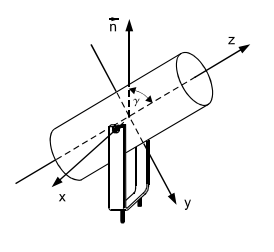
\includegraphics[width=200pt]{fotos/gpr1/Zylinder.png}			% einfügen des Bildes/ mit width Bildbreite einstellen
		\caption{verstellbarer Zylinder: $ \vec{n} $=Drehachse; x,y,z=Haupträgheitsmomente, wobei $ J_{x}=0 $ gesetzt wird; $ \gamma $ ist der Winkel, mit dem der Zylinder gedreht wird.}							% Bildunterschrift
		\label{Abb.: Zylinder}							% für Textverweise
	\end{figure}
	Ziel in diesem zweiten Teilversuch ist, das Trägheitsellipsoid zu überprüfen. Dies tun wir, indem wir die Linearität zwischen $ J _{\gamma} $ und $ \sin^{2}(\gamma) $ zeigen. Der Versuch mit dem Zylinder funktioniert ähnlich, wie der erste Teilversuch. Als erstes messen wir die Periodendauer der Halterung des Zylinders, wie sie in Abbildung (\ref{Abb.: Zylinder}) gezeigt wird, zweimal à 10 Perioden. Danach Setzen wir den Zylinder auf die Halterung, stellen $ \gamma \in [0^{\circ},90^{\circ}] $ in 15°-Schritten ein und messen die Periodendauer über 10 Perioden zweimal. Um $ J_{\gamma} $ zu bestimmen nutzen wir die Glg. (\ref{eq: T_sq=f(J_z)}) und stellen diese nach $ J_{Z} $ um:
	\begin{equation}\label{eq: J_Z}
		J_{Z}=\dfrac{D}{4\pi^{2}}T^{2}-J_{Tisch}
	\end{equation}
	Um aus $ J_{Z} $ $ J_{\gamma} $ zu bestimmen, nutzen wir folgende Gleichung:
	\begin{equation}\label{eq: J_gamma}
		J_{\gamma}=J_{Z}-J_{\text{Halterung}}
	\end{equation}
Für die Fehler von $ J_{Z} $ und $ J_{\gamma} $ nutzen wir wieder die Fehlerfortpflanzung, wie wir sie bereits in Glg. (\ref{eq: Fehlerfortpflanzung}) gezeigt haben.\\
Damit ergibt sich für $ J_{Z} $ ein Fehler von:
\begin{equation}\label{eq: J_Z_err}
	u_{J_{Z}}=\sqrt{\dfrac{u_{D}^{2}}{16\pi^{4}}T^{4}+2\dfrac{D^{2}}{16\pi^{4}}T^{2}u_{T}^{2}+u_{Tisch}^{2}}
\end{equation}
Der Fehler für $ J_{\gamma} $ setzt sich wie folgt zusammen:
\begin{equation}\label{eq: u_Gamma}
	u_{J_{\gamma}}=\sqrt{u_{J_{Z}}^{2}+u_{J_{\text{Halterung}}}} 
\end{equation}
	
	\section{Versuchdurchführung und Versuchauswertung}
	% übersichtliche Darstellung der Messdaten, Rechenergebnisse (chronologische Reihenfolge), Grafiken etc.
	
	
	
	\subsection{Bestimmung des Trägheitsmoments von einem Drehtisch}
	
    \begin{table}[H]
    \centering
		\caption[Versuch mit Scheibe]{Versuch mit Scheibe\\
			s ist der Abstand zwischen Drehachse A und Schwerpunkt, $ u_{s}=5\cdot 10 ^{-5} $ m, $ T_{1} $ ist die erste Periodendauer über 10 Schwingungen und $ T_{2} $ ist die zweite Periodendauer über 10 Schwingungen}
		\begin{tabular}{|c|c|c|}
			\hline
			s [m] & $ T_{1} $ [s] & $ T_{2} $ [s]\\
			\hline
			-- & 4.66$ \pm0.01 $ & 4.55$ \pm0.01 $ \\
			\hline
			$ 0$&4.96$ \pm0.01 $  & 4.98 $ \pm0.01 $\\
			\hline
			0.0112& 5.02$ \pm0.01 $ & 5.08$ \pm0.01 $ \\
			\hline
			0.0281& 5.53$ \pm0.01 $ & 5.70$ \pm0.01 $ \\
			\hline
			0.0417& 6.48$ \pm0.01 $ & 6.50$ \pm0.01 $ \\
			\hline
			0.0566& 7.51$ \pm0.01 $ & 7.32$ \pm0.01 $ \\
			\hline
			0.0714& 8.47$ \pm0.01 $ & 8.44$ \pm0.01 $ \\
			\hline
		\end{tabular}
		\label{Tab: J_Tisch}
\end{table}
    
	Für den ersten Teilversuch bekommen wir die Ergebnisse in Tabelle (\ref{Tab: J_Tisch}), wobei wir aus der Messreihe für $ s $ mithilfe der weiter oben in der Fußnote 2 erwähnten Radius und Masse der Scheibe mit dem steinerschen Satz (\ref{eq: J_Z1}) $ J_{Z} $ errechnen können.\\
	Die Regressionsparameter $ D $ und $ J_{Tisch} $ können wir dann mithilfe von \textit{scipy}, einem Python-Modul, bestimmen und kommen auf folgende Ergebnisse:
	\begin{align}
		D=(0.1036\pm 0.0025)\text{ mkg$ ^{2} $s$ ^{-2} $}\\
		J_{Tisch}=(5.8\pm 0.2)10^{-4} \textit{ mkg$ ^{2} $}
	\end{align}                                
	Weiterhin kommen wir für die lineare Regression$ ^{\ref{Abb.: J_Z} } $ auf ein
	\begin{equation}\label{eq: R_sq_tisch}
		R^{2}=0.999
	\end{equation}
	und auf ein 
	\begin{equation}\label{eq: chi_sq_tisch}
		\chi^{2}=2.5.
	\end{equation}
    Die lineare Regression zwischen $ T^{2} $ und $ J_{Z} $ befindet sich in Abb. (\ref{Abb.: J_Z}).\\
    Wir können mit großer Wahrscheinlichkeit sagen, dass zwischen $ J_{Z} $ und $ T^{2} $ ein lineare Beziehung existiert.
    
    \newpage
    \subsection{Überprüfung des Trägheitsellipsoids eines Zylinders}
    
    \begin{table}[H]
    \centering
    	\caption[Versuch mit Zylinder]{Versuch mit Zylinder\\
    		$\gamma$ ist der Auslenkwinkel des Zylinders, $ T_{1} $ ist die erste Periodendauer über 10 Schwingungen und $ T_{2} $ ist die zweite Periodendauer über 10 Schwingungen}
    	\begin{tabular}{|c|c|c|}
    		\hline
    		$\gamma$ [Grad] & $ T_{1} $ [s] & $ T_{2} $ [s] \\
    		\hline
    		0& 5.81$ \pm0.01 $  & 5.76$ \pm0.01 $  \\
    		\hline
    		15& 6.24$ \pm0.01 $ & 6.28$ \pm0.01 $  \\
    		\hline
    		30& 6.50$ \pm0.01 $  & 6.46$ \pm0.01 $  \\
    		\hline
    		45& 7.11$ \pm0.01 $  &7.06$ \pm0.01 $   \\
    		\hline
    		60& 7.66$ \pm0.01 $  &  7.63$ \pm0.01 $ \\
    		\hline
    		75	& 8.04$ \pm0.01 $  &  8.02$ \pm0.01 $ \\
    		\hline
    		90& 8.13$ \pm0.01 $  & 8.11$ \pm0.01 $  \\
    		\hline
    	\end{tabular}
    	\label{Tab: sin}
\end{table}
    
    Die Messergebnisse der zweiten Teilversuch sind in der neben dran. 
    Für die Regressionsgeraden in Abb. (\ref{Abb.: gam}) haben wir die folgende Form verwendet:
    \begin{equation}\label{eq: allg_Reg.gerade}
    	J_{\gamma}=a\cdot \sin^{2}(\gamma)+b.
    \end{equation}
	Diese ist mit der folgenden Gleichung aus dem verlinkten Skript \textbf{M2 Trägheitsmomente} äquivalent:
	\begin{equation}\label{eq: gamma}
		J_{\gamma}=J_{z}+(J_{y}-J_{z})\sin^{2}(\gamma).
	\end{equation}
	Für Fitparamter $ a $ und $ b $ haben wir folgende Ergebnisse:
	\begin{align}
		a=(-2.7\pm0.2)10^{-4} \text{ m(kg)$ ^{2} $}\\
		b=(8.2\pm0.4)10^{-4} \text{ m(kg)$ ^{2} $}
	\end{align}
\\
Daraus lassen sich nach Glg. (\ref{eq: gamma}) für 
\begin{align}
	J_{z}=(8.2\pm0.4)10^{-4} \text{ m(kg)$ ^{2} $}\\
	J_{y}=(-10.9\pm0.4)10^{-4} \text{ m(kg)$ ^{2} $}
\end{align}
errechnen. Dabei ist $ J_{z} $ das Trägheitsmoment des Zylinders mit einer Auslenkung von $ 0^{\circ} $ und $ J_{y} $ ist das Trägheitsmoment des Zylinders bei $ 90^{\circ} $. \\
Betrachten wir nun die theoretischen Werte von $ J_{z} $ und $ J_{y} $. Diese errechnen wir mit den geometrischen Werten und der Masse des Zylinders.\footnote{Radius: $ R=(205.00\pm0.25)10^{-4} $ m, Höhe: $ h=(1010.00\pm 0.5)10^{-4} $ m, Masse: $ m=(1352.0\pm 0.1)10^{-3} $ kg} Die Ergebnisse lauten wie folgt:
\begin{align}
	J_{z}=(2.841\pm 0.007)10^{-4} \text{ m(kg)$ ^{2} $}\\
	J_{y}=(12.914\pm 0.012)10^{-4}\text{ m(kg)$ ^{2} $}
\end{align}
Vergleichen wir die theoretischen Werte mit den Werten aus der Regression, so passen diese nicht über ein und wir können keine Aussage darüber geben, ob das Modell der Linearität zwischen $ J_{\gamma} $ und $ \sin^{2}(\gamma) $ richtig ist oder nicht.
	
\newpage
	\section{Diskussion}
	% Diskussion über Versuchsergebnisse und Versuchsaufbau
	% gründliche Analyse der aufgetretenen Messabweichungen und ihre Ursachen
	% ergebnisse mit Referenzwerten unter angaben von Quellen vergleichen
	% Angabe von Messunsicherheiten und ihre Berechnung bzw. Abschätzung
	% experimentele Methoden und Messverfahren  kritisch beobachten und diskutieren, Schlussfolgerungen gezogen werden
	% Resumé bzw. eine kurze Zusammenfassung
	\subsection{Trägheitsmoment des Tisches}
	Wir konnten im ersten Teilversuch einen linearen Zusammenhang zwischen $ T^{2} $ und $ J_{Z} $ feststellen. Diesen zeigt die lineare Regression in der Abb. (\ref{Abb.: J_Z}). Eine differenzierte Fehleranalyse ist nicht möglich, da wir beispielsweise die Reaktionszeit des Experimentators nicht gemessen haben und konnte dieser Fehler auch nicht mit einfließen. Trotzdem können wir davon ausgehen, dass wir den Daten vertrauen können.
	
	\subsection{Trägheitsmoment des verstellbaren Zylinders}
	Der Fit in der Abb. (\ref{Abb.: Zylinder}) passt nicht mit den Datenpunkten überein. Dies sieht man auch an dem $ \chi^{2} $, welches wir in der Beschreibung angegeben haben, sieht, da dieses extrem groß ist. Vergleicht man in diesem Zuge die theoretischen Trägheitsmomente mit denen die aus der Regression errechnet wurden, so stimmen diese nicht über ein. Dies lässt darauf schließen, dass wir einen groben Messfehler begangen haben. Nach einigen Überlegungen, wo der grobe Messfehler begangen wurde, sind wir zu dem Schluss gekommen, dass dieser wohl in dem Ablesen der Winkel liegt. Hierzu gibt es zwei wichtige Einflüsse: Zum einen hatte der Experimentator eine etwas niedrige Konzentration aufgrund der Tageszeit (Zeitraum: ~ 16.30-17.00 Uhr) und zum anderen ist die leichte Sehschwäche des Experimentators zu erwähnen. Dieser trug seine Brille nicht, mit der Begründung, dass die Brille mit der Maske, die wir aufgrund der Corona-Pandemie tragen müssne, dafür gesorgt hätte, dass die Brille beschlagen wäre und ein korrektes Ablesen der Winkel deutlich erschwert hätte. Zudem können wir uns nicht sicher sein, dass die Winkel in den oben genannten Winkel (Tabelle (\ref{Tab: sin})) mit denen übereinstimmen, die wir abgelesen haben, da wir diese nicht persönlich gemessen haben und die Winkel waren auch nicht angegeben. \\
	Wir kommen zu dem Schluss, dass den Daten aus dem zweiten Teilversuch aus genannten Gründen nicht zu vertrauen ist.
	
	\newpage
    \appendix
	\section{Anhang}
	\subsection{Abbildungen}
	\begin{figure}[!ht]
		\centering									% Bild Zentrierung
		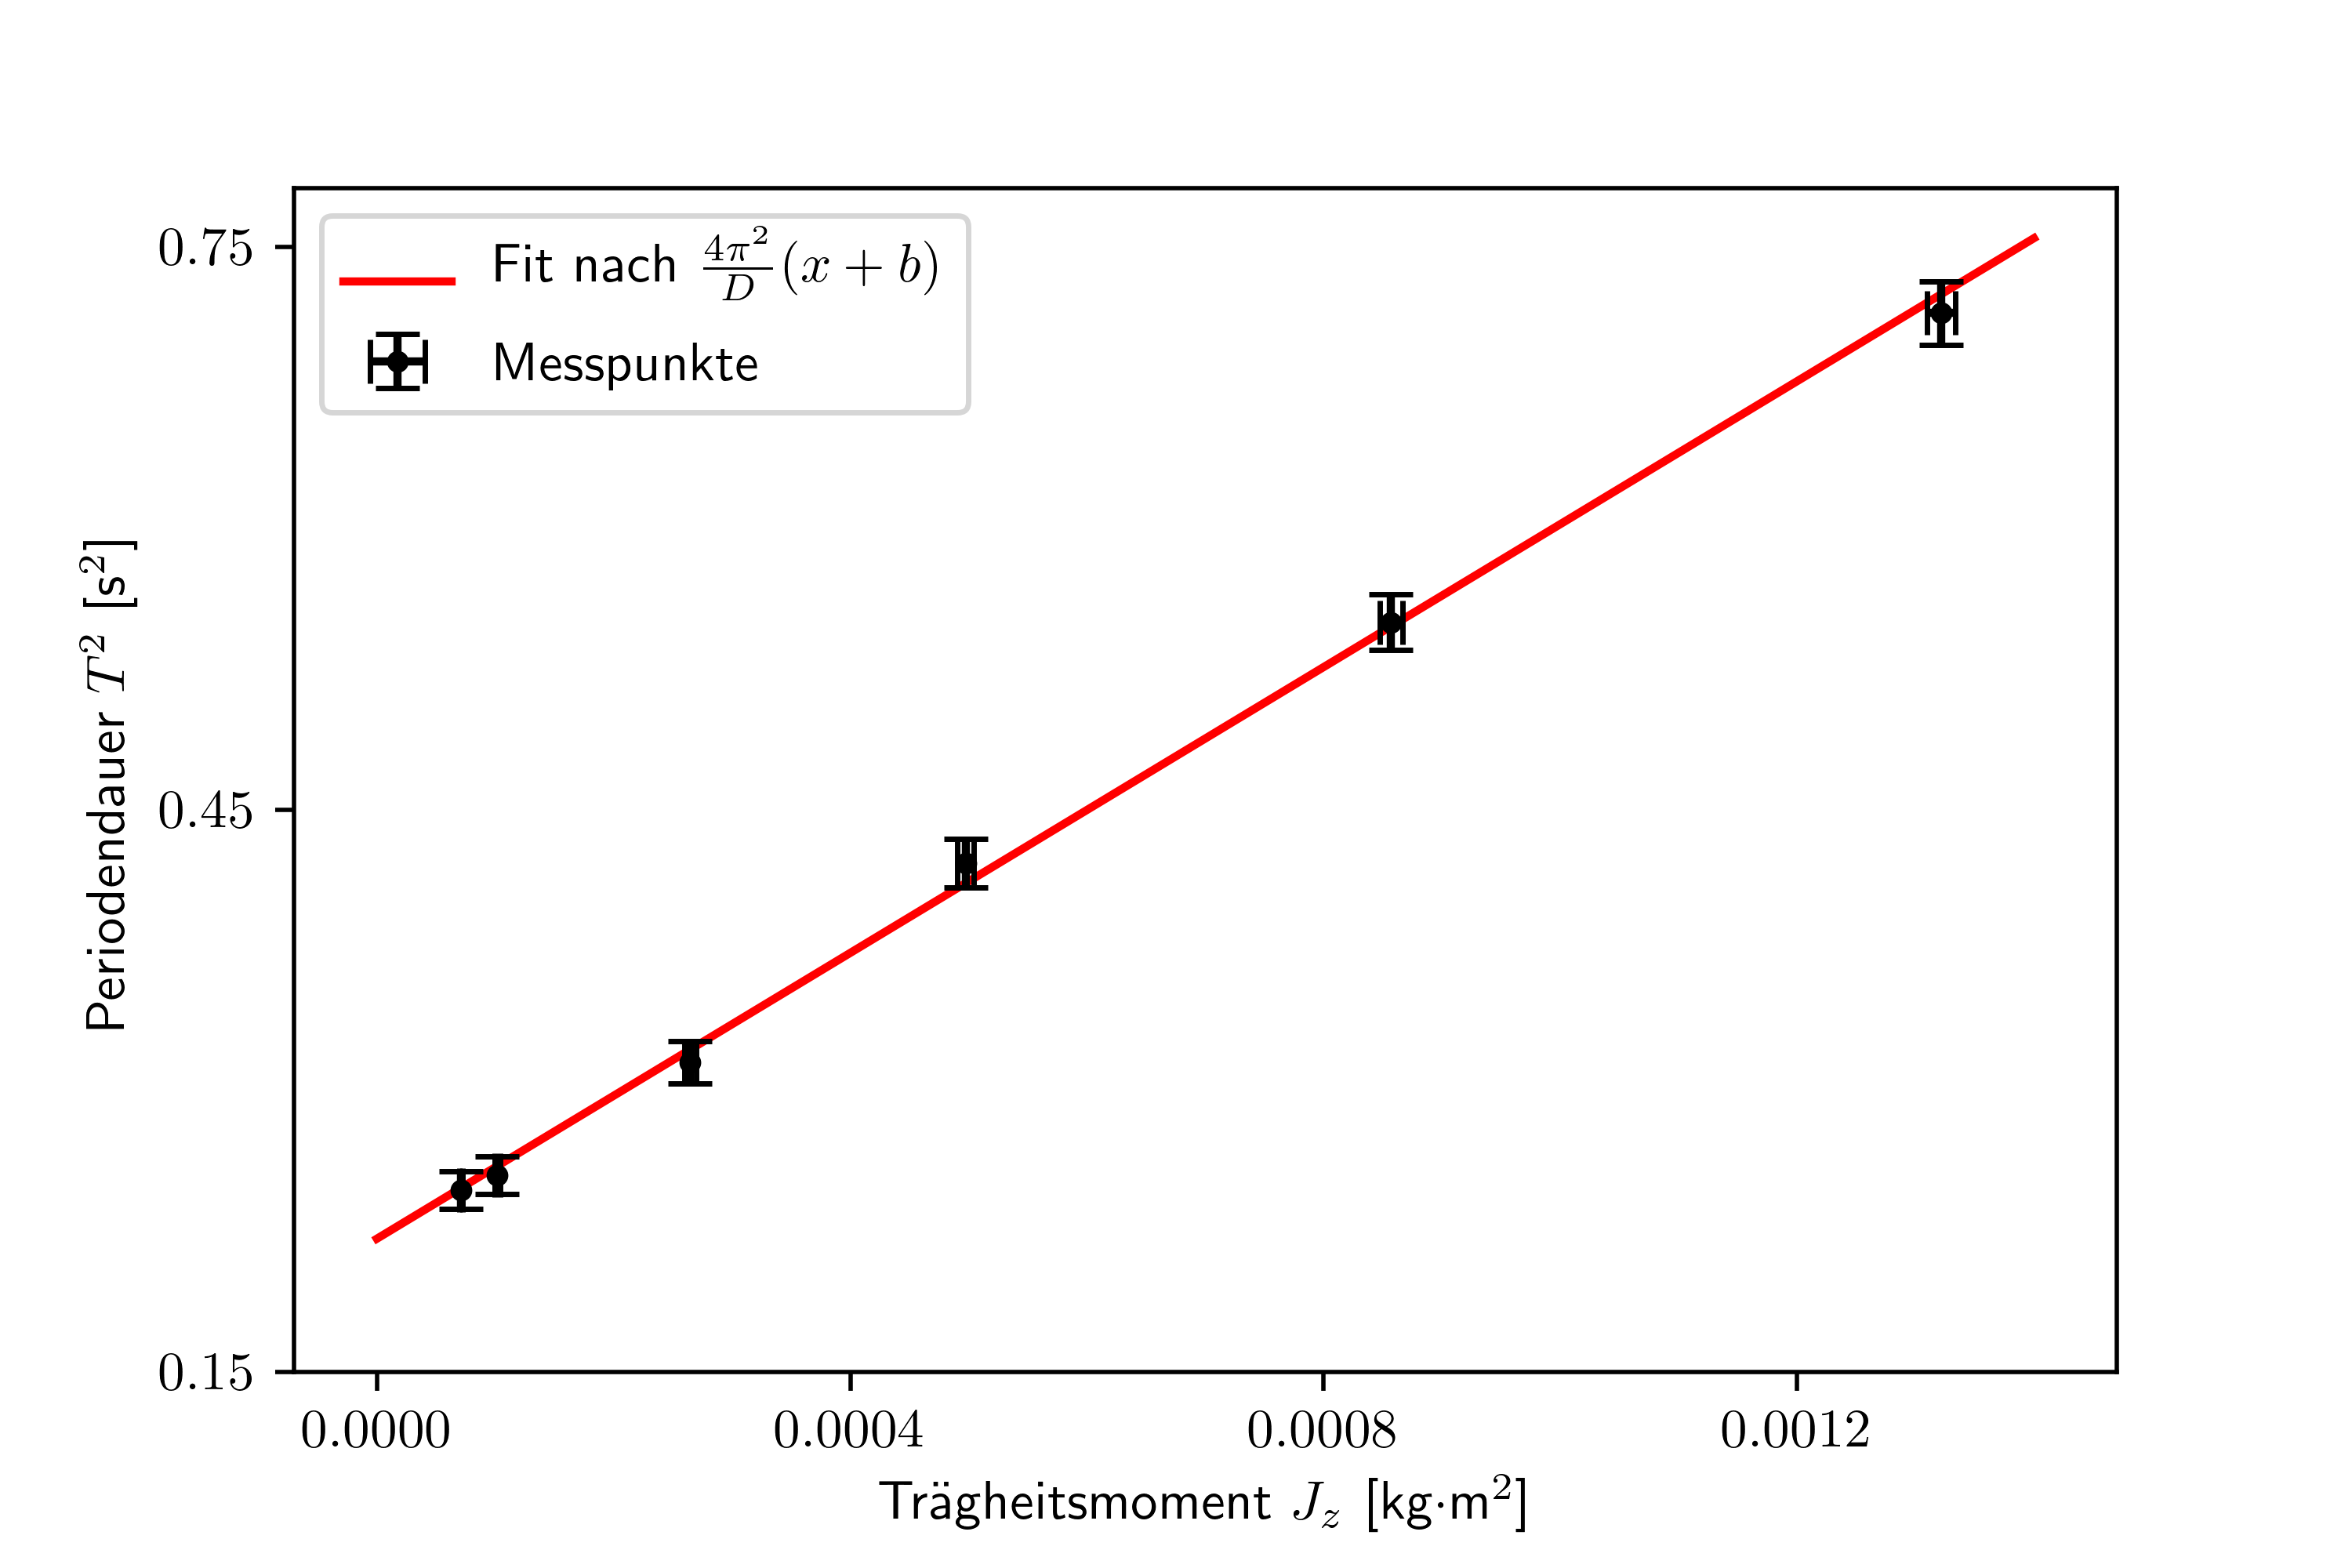
\includegraphics[width=300pt]{fotos/gpr1/Regression_M2_J_Tisch.png}			% einfügen des Bildes/ mit width Bildbreite einstellen
		\caption{Linearität zwischen quadrierter Periodendauer $ T^{2} $ und Trägheitsmoment $ J_{Z} $. Fehlerbalken sind durch Fehlerfortpflanzung entstanden. Abbildung zeigt gemittelte Werte für $ T^{2} $ aus der Tabelle (\ref{Tab: J_Tisch}). $ R^{2}=0.999 $. $ \chi^{2}=2.50 $ }							% Bildunterschrift
		\label{Abb.: J_Z}							% für Textverweise
	\end{figure}

\begin{figure}[!ht]
	\centering									% Bild Zentrierung
	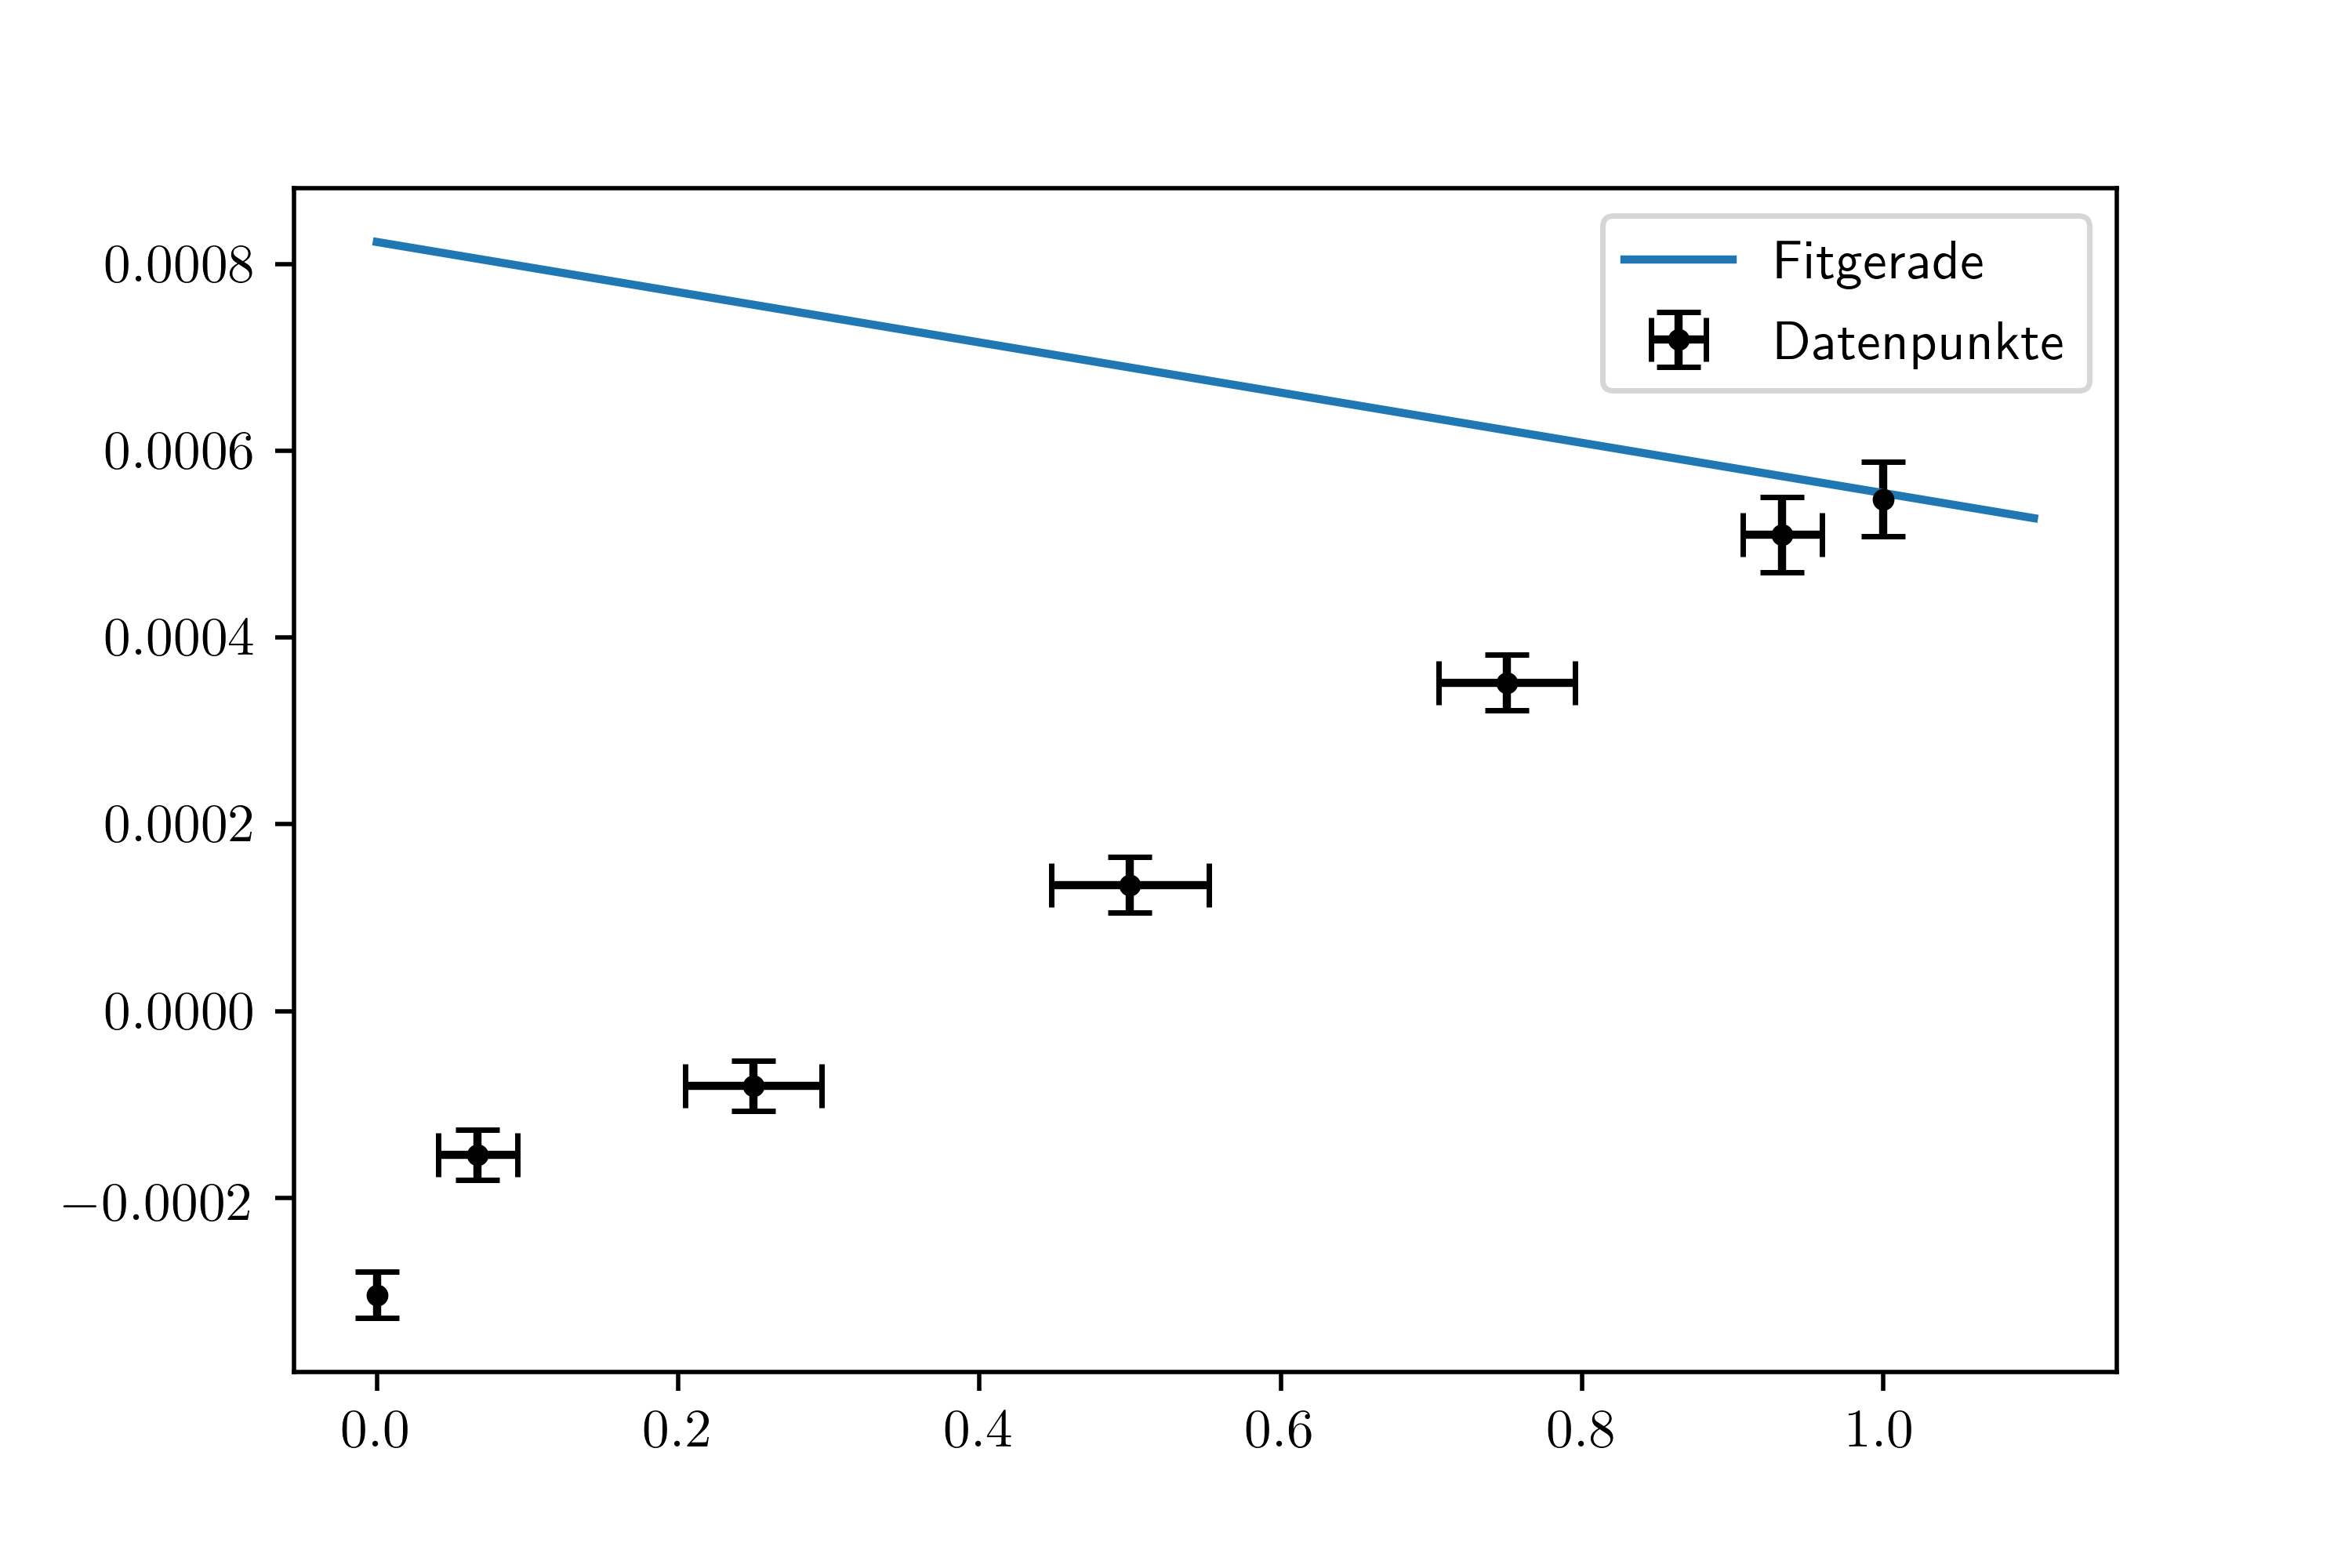
\includegraphics[width=300pt]{fotos/gpr1/Regression_Zylinder.png}			% einfügen des Bildes/ mit width Bildbreite einstellen
	\caption{Linearität zwischen $ J_{\gamma} $ und $ \sin^{2}(\gamma) $. Abbildung zeigt gemittelte Werte von $ T^{2} $ aus der Tabelle (\ref{Tab: sin}). $ R^{2}=0.992 $, $ \chi^{2}=6164.4 $ }							% Bildunterschrift
	\label{Abb.: gam}							% für Textverweise
\end{figure}
	
	\newpage
	
	\printbibliography[title={Quellenverzeichnis}]
	
	
\end{document}